\section{Laboratory work implementation}

\subsection{Tasks and Points}

\begin{itemize}
	\item Realizeaza un site cu folosirea maximala a tagurilor
	\item Pentru formatarea paginilor se va folosi CSS
	\item Site-ul trebuie sa pastreze toata informatia intr-o baza de date
	\item Site-ul trebuie sa contina AJAX Requests.
	\item Implimentarea XHR sau JSON responses. Careva din informatie trebuie sa fie dinamic incarcata pe pagina.
\end{itemize}

\subsection{Analiza lucrarii de laborator}
Repository \href{https://github.com/nadejda-danart/TI-141-F-R-MIDPS/tree/master/laborator3}{link}\par


În această lucrarea de laborator am elaborat un website de tip visit card, a unei companii ce oferă servicii de design interior și exterior a încăperilor/caselor, în care sunt 2 compartimente: Prima pagină(Home Page) și Portofoliu.

\subsubsection{Home page}

Prima pagină și este cartea vizită așa cum conținutul rezumativ se află în ea:

\begin{itemize}
	\item Mesajul de bun venit
	\item Portofoliu
	\item Interioarele finalizate
	\item Clienții noștri
	\item Publicitate
	\item Echipa
	\item Metode de contact
\end{itemize}

Mesajul de bun (referință: \ref{welcome}) venit contituie într-un mic video care se află pe fundalul aplicației ca "background", care este poziționate într-un tag de tip <div> care are o poziție abosolută și z-index (poziția pe axa z într-un spațiu 3D) - -1 pentru a nu astupa restul contentului și anume mesajul de bun venit, care la rândul său a fost centrat cu stilul text-align. Din compartimentul dat avem o săgeată care ne duce lin spre urmatorul comparitiment printr-o animație făcută de către librăria JQuery\cite{jquery}.

Portofoliu (referință: \ref{portfolio}) este compus din 9 imagini, exemple de lucru a companiei, care au fost centrate cu sistema de grid oferită de librăria bootstrap\cite{boostrap}, iar sursa lor provine de la server care ne returnează ultimele 9 lucări. Apelarea serverului a avut loc de asemenea prin intermediul comenzii \$.get()\cite{get-method} care de asemnea este oferită de librăria JQuery. Fiecare imagine are un eveniment atârnat față de ele de tip hover care ne permite mărirea cu stilul transform:scale și apariția textului cu stilul opacity: 1 (referință: \ref{scaled}).

Interioarele finalizate (referință: \ref{finalized}) constă în 2 clipulețe video, iar codul pentru ele a fost oferit de YouTube, doar leam centralizat de asemenea cu ajutorul librăriei bootstrap.

Clienții nostri (referință: \ref{clients}) este compartimentul unde am afișat lista clienților. Am adăugat un background cu poziția fixă ce crează o iluzie plăcută în timp ce facem scroll.

Publicitatea (referință: \ref{ad}) e un video clip scurt în care se explică beneficiile companiei.

Echipa (referință: \ref{team}) constă în afișarea personalului curenta care la fel are un background fix.

Compartimentul Metode de contact (referință: \ref{contact}) are o formă în care utilizator își scrie datele lui pentru al contacta și întrebarea sau mesajul care dorește să îl acorde comapniei. După completarea formei prin intermediul comenzii \$.post() se trimite un request serverul care salvează în bază de date această informație. La finisarea completării și trimiterea mesajului forma dispare și apare un mesaj care mulțumeste clientul.

\subsubsection{Portfolio}

Pagina portofoliu (referință: \ref{portfolio-original}) constă într-o listă de imagini a tuturor lucrărilor făcute de companie. Aceste imagini la fel sunt primite din partea serverului. Imaginile curente au aceleași evenimente ca și în preview care ne permite vizualizarea denumirii proiectului.


\subsubsection{Menu}

Meniul aplicației web (referință: \ref{menu-up}) are și el o funcționalitate de ași schimba înfățișarea când poziția pe pagina pe pagină nu mai este cea de sus (referință: \ref{menu-moved}). Acest funcțional a fost adăugat la evenimentul scroll a documentului.

\subsubsection{Server}

Pentru pornirea unui server am folosit unul din puțin cunoscutul framework NodeJS\cite{nodejs}, care limbajul de programare tot este JavaScript. Am conectat modulul Express\cite{expressjs} care permite ridicarea serverului și crearea unor endpoints.
Prin intermediul lui citeam toate imaginile dintr-un fișier și pe baza de metadata lor le ordonam pentru a trimite 9 cele mai noi imagini. Denumirea proiectelor era și denumirea fișierelor. Pentru citirea imaginilor am folosit modului FileSystem care este inclus in NodeJS.

Ca baza de date am folosit una nerelațională LokiJS\cite{lokijs} în care salvez toate întrebările și mesajele clienților trimise din website.

\subsection{Imagini}
\begin{center}	
	\begin{figure}[h]
		\centering
		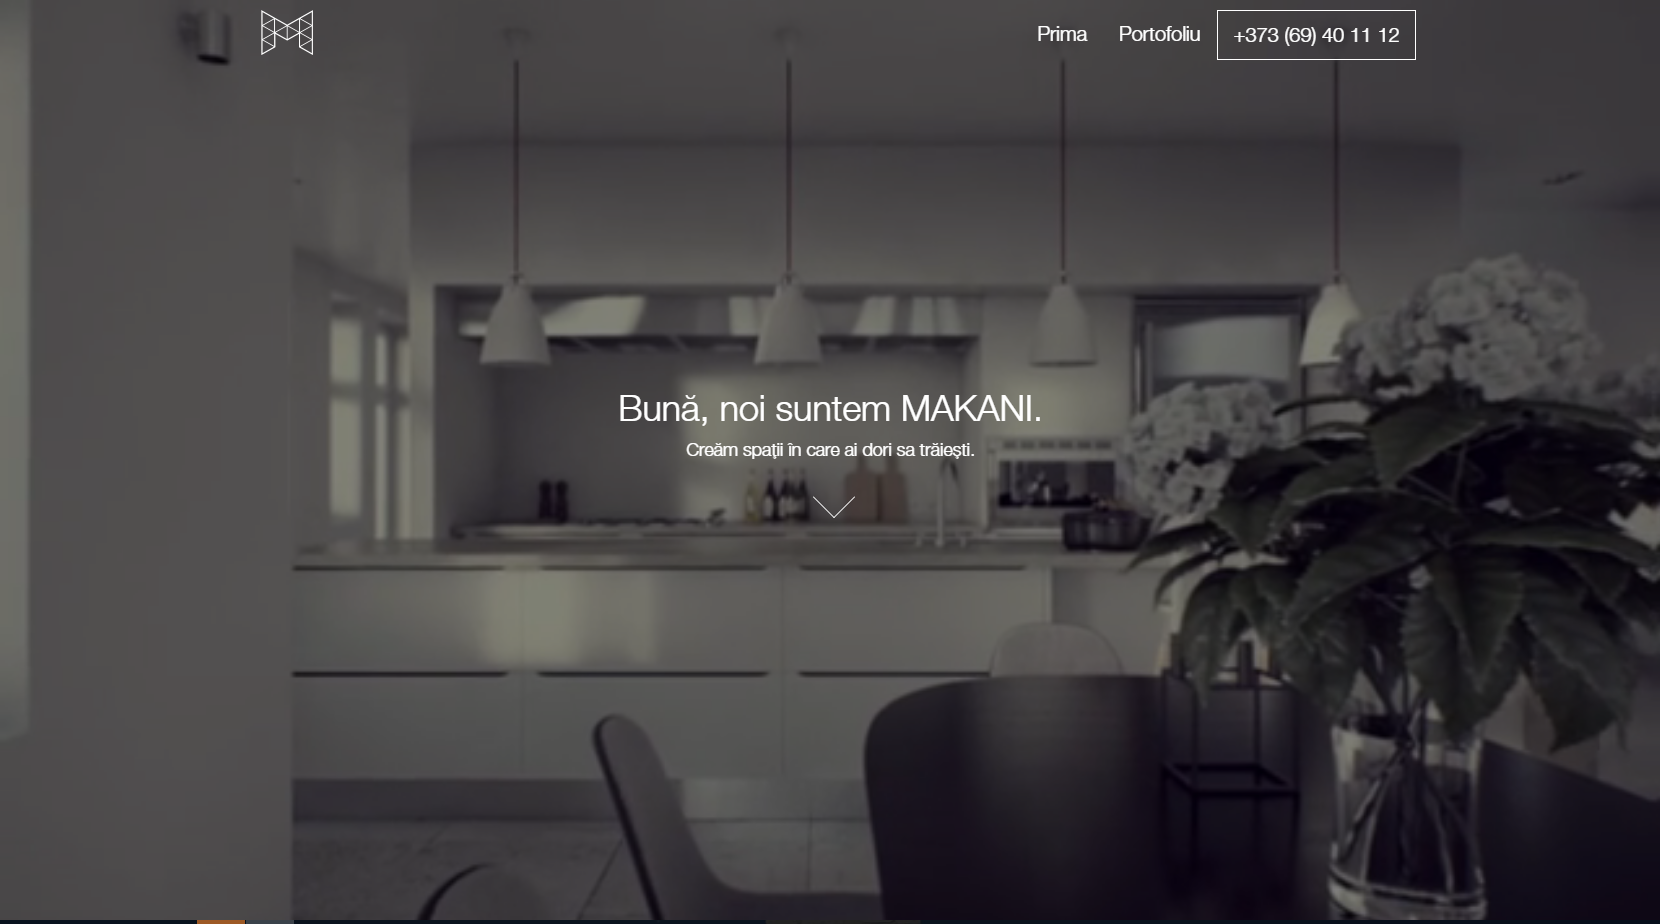
\includegraphics[width=15cm]{welcome}\\
		\caption{Welcome part of the page}
		\label{welcome}
	\end{figure}
	
	\begin{figure}[h]
		\centering
		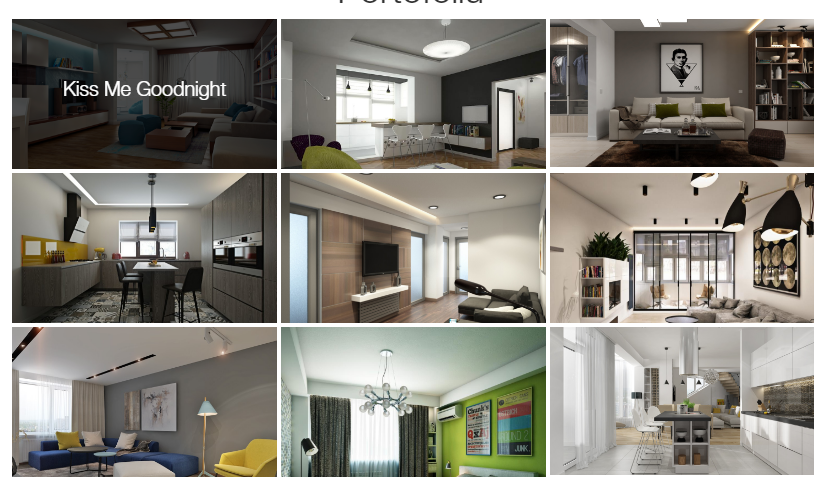
\includegraphics[width=15cm]{scaled}\\
		\caption{Scaled portfolio preview}
		\label{scaled}
	\end{figure}
	
	\begin{figure}[h]
		\centering
		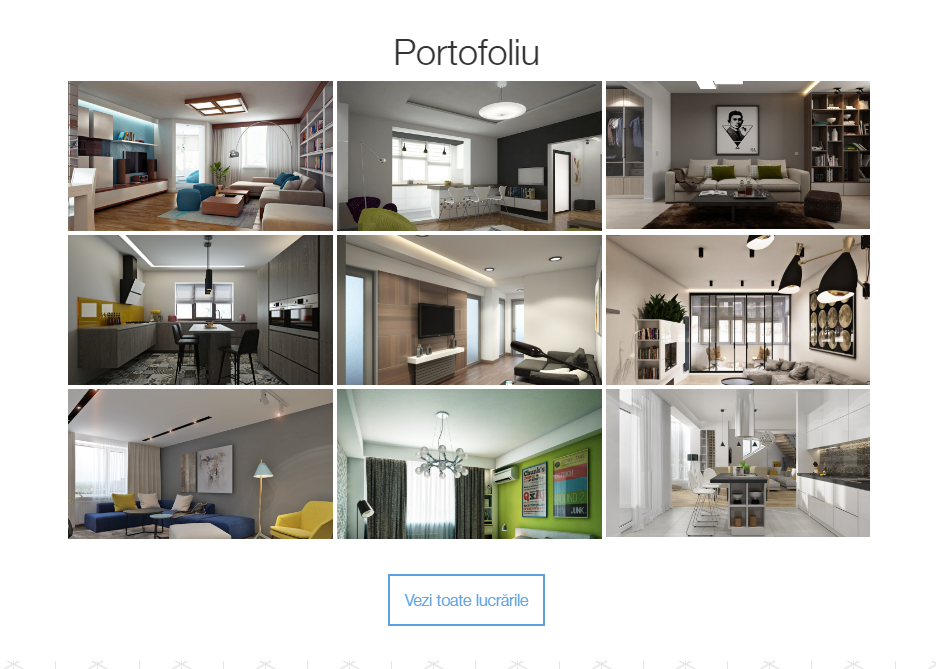
\includegraphics[width=15cm]{portfolio}\\
		\caption{Portfoliu preview}
		\label{portfolio}
	\end{figure}
	
	\begin{figure}[h]
		\centering
		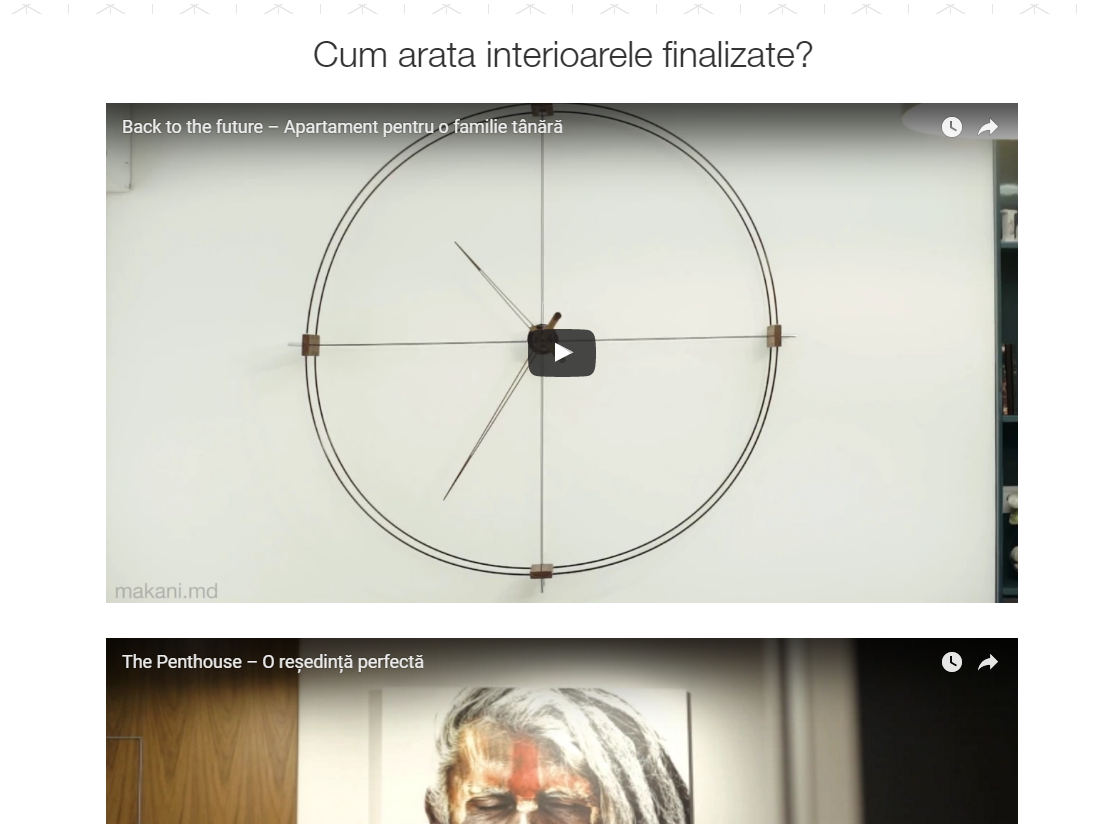
\includegraphics[width=15cm]{finalized}\\
		\caption{Finalized works}
		\label{finalized}
	\end{figure}
	
	\begin{figure}[h]
		\centering
		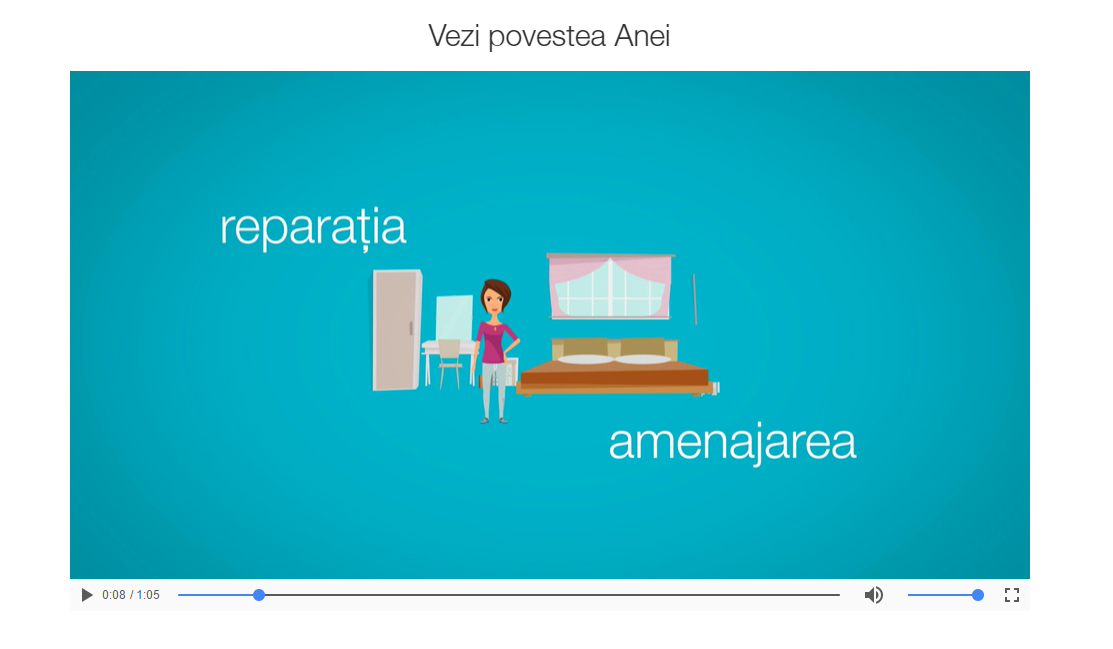
\includegraphics[width=15cm]{ad}\\
		\caption{Ad of the company}
		\label{ad}
	\end{figure}
	
	\begin{figure}[h]
		\centering
		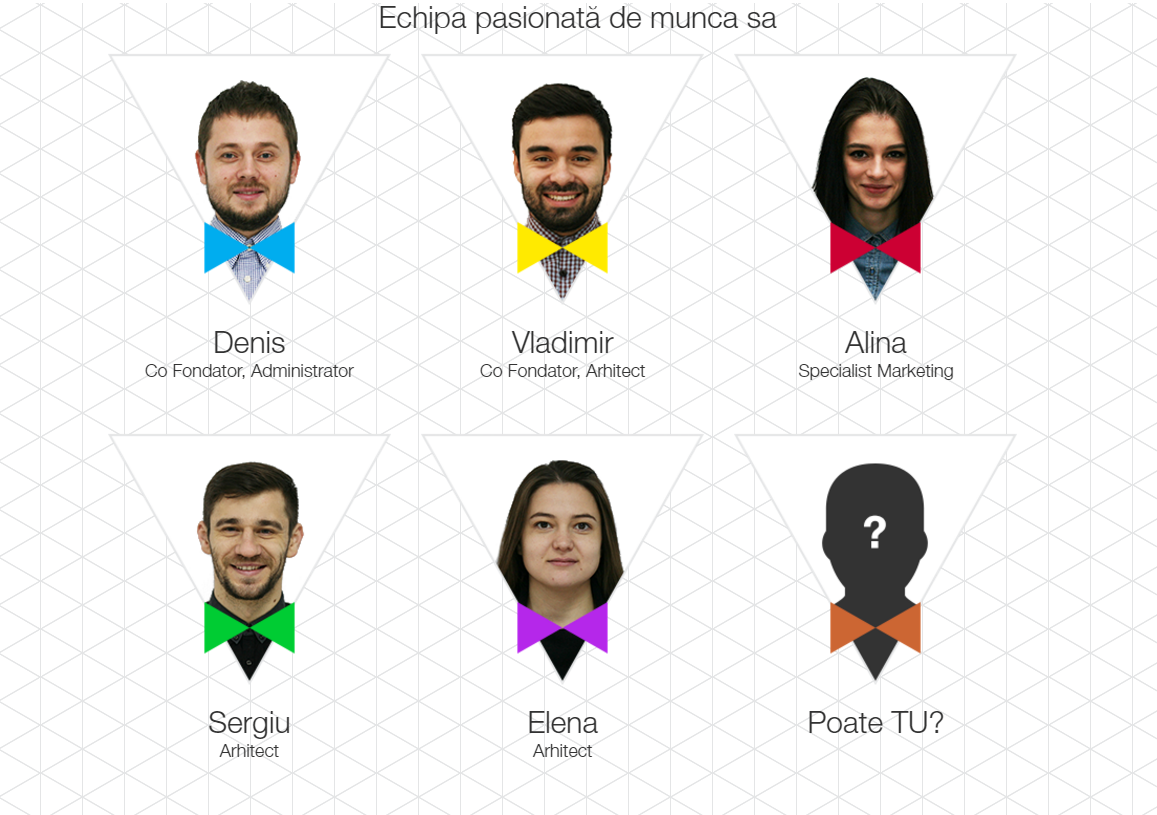
\includegraphics[width=15cm]{team}\\
		\caption{Team}
		\label{team}
	\end{figure}
	
	\begin{figure}[h]
		\centering
		
\includegraphics[width=15cm]{clients}\\
		\caption{Clients list}
		\label{clients}
	\end{figure}
	
	\begin{figure}[h]
		\centering
		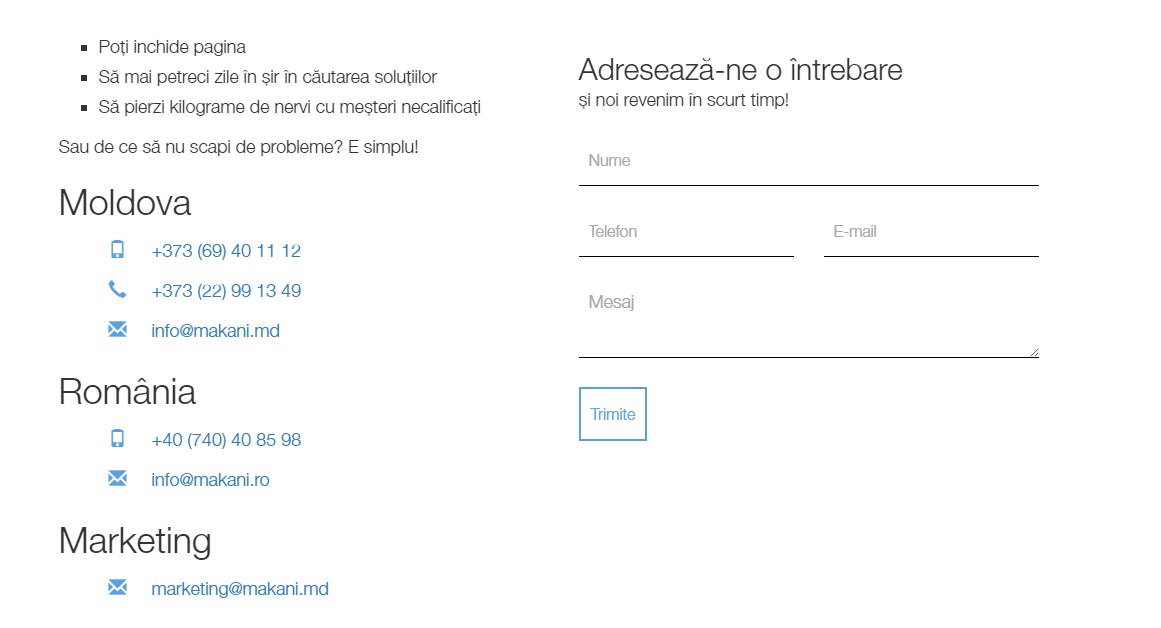
\includegraphics[width=15cm]{contact}\\
		\caption{Contact us}
		\label{contact}
	\end{figure}
	
	\begin{figure}[h]
		\centering
		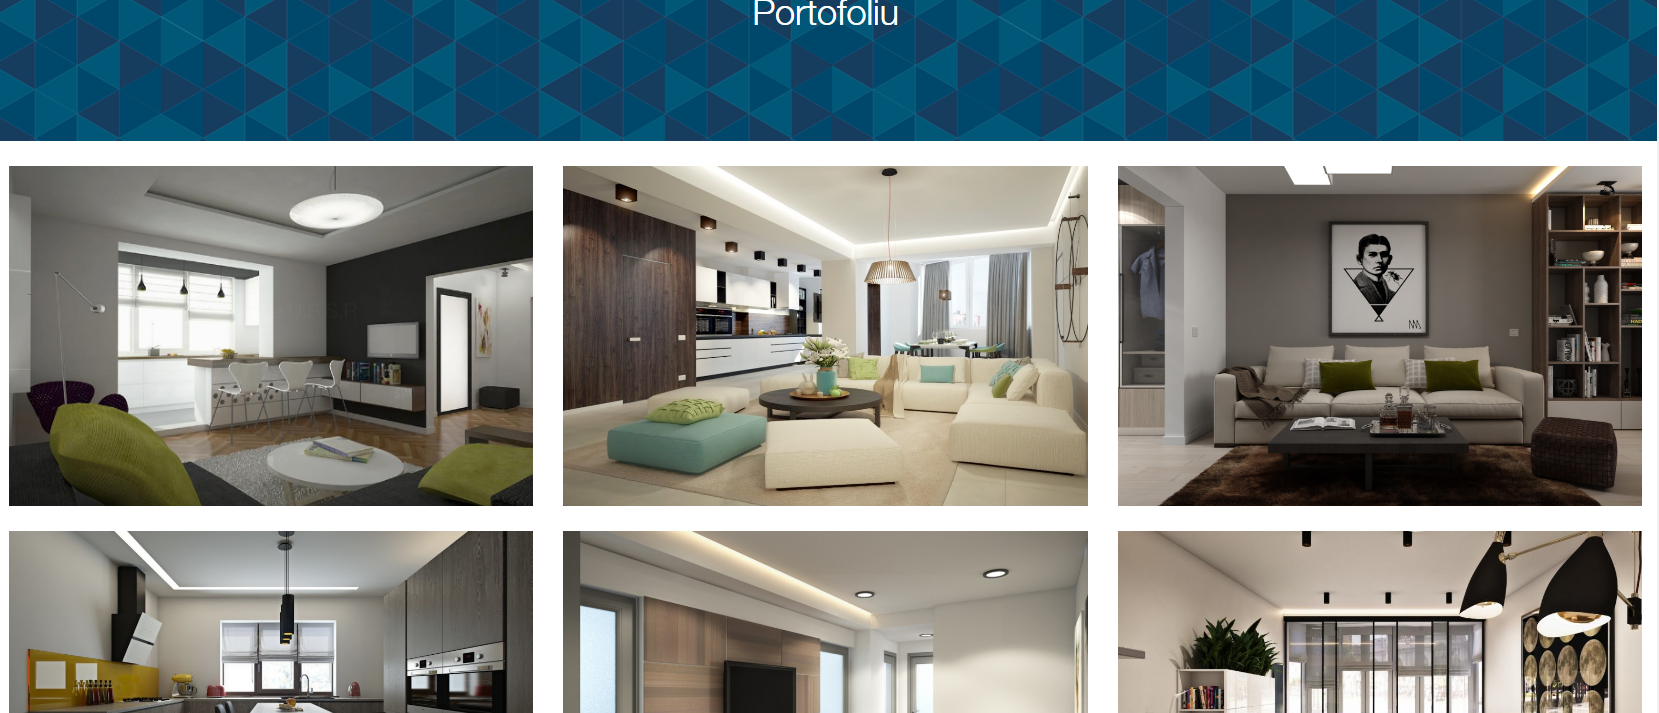
\includegraphics[width=15cm]{portfolio-original}\\
		\caption{Full portfolio}
		\label{portfolio-original}
	\end{figure}
	
	\begin{figure}[h]
		\centering
		
\includegraphics[width=15cm]{menu-up}\\
		\caption{Menu original state}
		\label{menu-up}
	\end{figure}
	
	\begin{figure}[h]
		\centering
		
\includegraphics[width=15cm]{menu-moved}\\
		\caption{Menu moved state}
		\label{menu-moved}
	\end{figure}
\end{center}

\clearpage